Este capítulo tem por objetivo detalhar os aspectos do desenvolvimento
do protótipo. Sua mecânica, o loop de eventos, diagramas entre outros
aspectos serão tratados aqui.

\section{MECÂNICA}

Para a análise prática das limitações foi escolhido um jogo de
matemática simples. Consistindo na geração de equações com uma
resposta candidata. Cabe ao usuário informar se o resultado apontado
pelo jogo está correto ou não. A cada resposta dada o nível de
complexidade da equação cresce. O tempo é um fator determinante
no resultado do jogo pois quão mais rápido o jogador acertar se a
afirmação está correta ou não mais pontos ele receberá.

Esta categoria de jogo foi selecionada por ter profundidade, oferecendo
a possibilidade de explorar diversos recursos do HTML, e criar melhorias
incrementais. E também por oferecer uma dificuldade técnica não
tão desafiadora visto que não disponho de experiência profunda no
desenvolvimento de jogos em HTML.

Jogos como o Math Workout e o Countdown para Android tem uma temática
similar. Não obstante, o Math Workout não apresenta a resposta, sendo
o papel do usuário computar a equação e digitar o resultado. Já o jogo
Countdown apresenta um número final e requer que o usuário determine
a equação que resultou no valor à partir de um dado conjunto de
números e operadores.

O jogo desenvolvido para o protótipo parece ter uma melhor jogabilidade
em dispositivos móveis que ambos os jogos acima citados pois não
requer a presença de um teclado numérico. Os botões de verdadeiro
ou falso contém todas as possibilidades. A figura \ref{fig:gameScreen}
demonstra a interface contendo com os botões.

Abaixo são descritos os requisitos que uma mecânica como a descrita 
acima deve prover.
%Também para não interferir na pesquisa busquei não me distanciar do
%que é considerado padrão em ferramentas e métodos.

\section{Requisitos}

Abaixo estão dispostos os requisitos do sistema.

\subsection{Requisitos funcionais}

As funcionalidades que o sistema deve apresentar estão descritas abaixo.

\begin{itemize}
    \item O sistema deve prover equações matemáticas de dificuldade crescente para o usuário informar se estão corretas ou não.
    \item O sistema deve pontuar as respostas dadas com maior agilidade com uma pontuação maior, que as respondidas com menor agilidade.
    \item O sistema deve apresentar um ranking com os resultados dos  jogos anteriores.
\end{itemize}

\subsection{Requisitos não funcionais}

Outros aspectos requisitados mas que todavia não fazem parte da regra de negócio.

\begin{itemize}
    \item O sistema deve ser desenvolvido utilizando as ferramentas da web.
    \item O sistema deve funcionar para a plataforma desktop e Android.
    \item O sistema deve ser desenvolvido sem a utilização de nenhuma biblioteca ou framework.
\end{itemize}

\section{Modelagem}

Abaixo segue o diagrama de classes simplificado \footnote{Nos anexos pode-se encontrar a versão completa do diagrama de classes}.

\begin{figure}
    \centering
    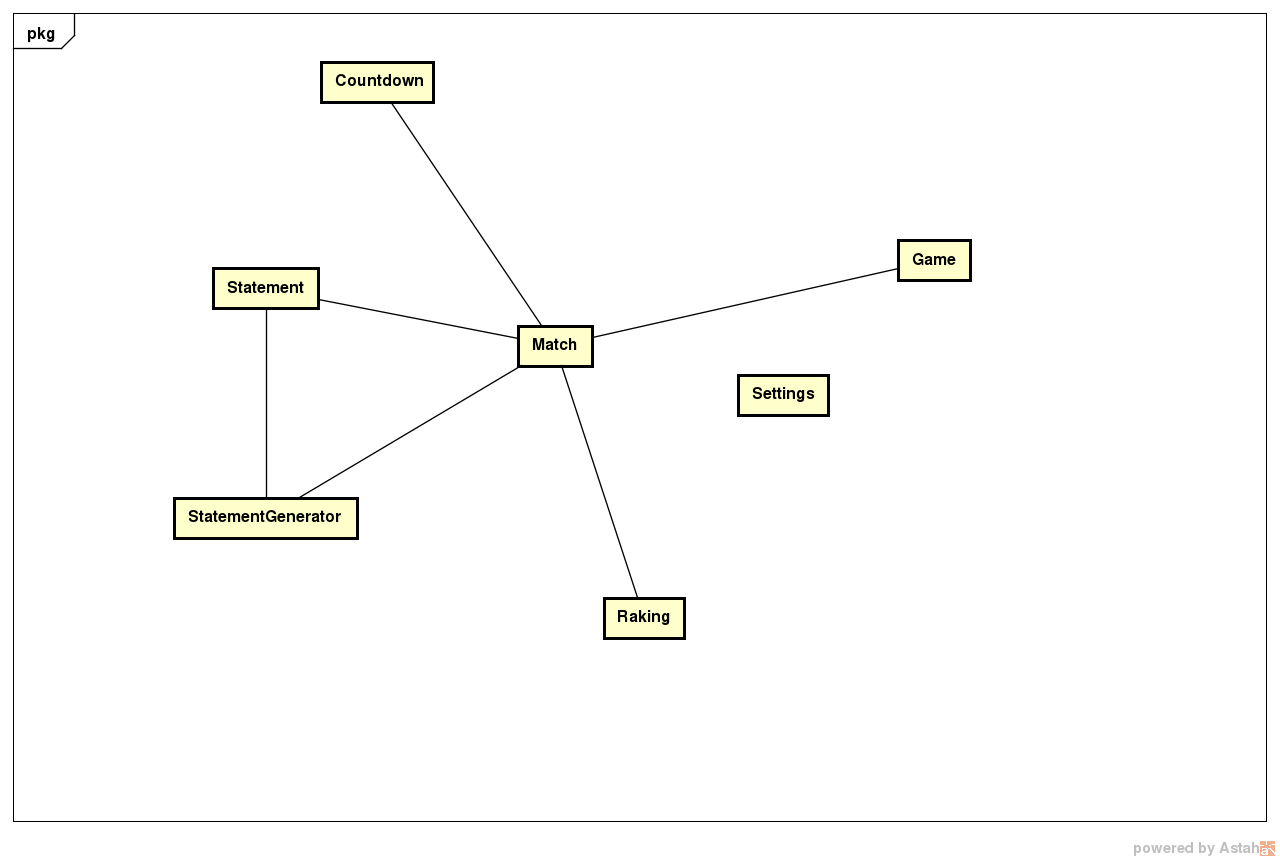
\includegraphics[width=0.8\textwidth,natwidth=610,natheight=642]{ClassesSimpleView.png}
	\caption{Diagrama de classes simplificado}
    \label{fig:simpleDiagram}
\end{figure}

\section{Desenvolvimento}
%Comecei escrevendo o aplicativo para o Navegador do desktop pois era o
%que estava mais acessível no momento.

O desenvolvimento se deu com uma postura de melhoria progressiva.
Desenvolvendo a versão mais simples possível para atingir as
requisitos funcionais. A partir dessa versão, novos recursos foram
sendo adicionadas para melhorar a experiência do usuário. Iniciei o
desenvolvimento criando para a plataforma Desktop pois esta contém
um grande número de ferramentas de desenvolvimento nativas que não
requerem integração especial.

O primeiro passo foi a criação do documento HTML. Utilizei divs
para simbolizar telas do jogo. Conter todas as telas em único
HTML caracteriza o jogo como uma aplicação de uma única página
(\textit{Single Page Application}). Alternativamente poderia se depender
de um servidor para mandar as páginas prontas, mas isso distribui
a complexidade do sistema para tecnologias do lado do servidor,
distanciando-se da proposta de jogos exclusivamente construídos com as
tecnologias da WEB.

Seguindo a construção do documento HTML, veio o desenvolvimento de um
CSS simples que comporta a visualização em múltiplos dispositivos.
Para tal, foram utilizadas posições e tamanhos relativos. Por exemplo,
a largura de cada tela da SPA é 98\% do tamanho total disponível na
tela. Já o tamanho da fonte do quadro principal, representado pelo id
\textit{billboard} é duas vezes o tamanho da fonte normal 2em.

Sem a ajuda de bibliotecas especializadas o processo de criação da
interface não é trivial. Apesar dela ser simples, fazer os
elementos se alinharem em diversos tamanhos de telas não é fácil e
pode se tornar um grande problema para interfaces realmente complexas.

Após a concepção do CSS deu-se início ao desenvolvimento da lógica
das páginas em JavaScript. O primeiro passo consistiu em fazer o
mecanismo de múltiplas telas em um único arquivo HTML através de JavaScript. Os
botões que levam a outras telas, quando clicados, simplesmente escondem
todas as seções e por fim carregam a que querem mostrar. Aplicativos
SPA introduzem outros desafios, por exemplo o botão de voltar
perde sua utilização visto que não se está trafegando de uma página
a outra de fato. HTML5 provê uma API em JavaScript para manipular o histórico
que pode resolver este problema; não obstante, no protótipo não
adicionamos esta funcionalidade pois a quantidade de telas é realmente
baixa e os benefícios introduzidos seriam baixos.

Ao iniciar a execução do JavaScript todas as divs que representam
telas são escondidas e a div de carregamento de recursos é mostrada em
seguida. No final do carregamento de todos os recursos é disparado o
evento \textit{window.onload} neste momento carrega-se a div da partida
e dá-se início a ela. Durante esta fase do desenvolvimento também
foram adicionados \textit{listeners} aos demais elementos interativos do
jogo, como clicar nas configurações e nos botões de certo e errado da
página principal.

Após o esqueleto da aplicação estar definido foi introduzido a
lógica de negócio. A figura \ref{fig:simpleDiagram} apresenta do
a relação entre as classes do jogo. De toda a regra do jogo, a
classe Match é a mais importante. Ela simboliza uma partida dentro do
jogo, é na classe Match que as informações de quantas equações
existem, quantas foram acertadas e o tempo total da partida bem como
sua pontuação atual. O propósito da classe Match é iterar a cada
pergunta e esperar por uma resposta. Quando a resposta é dada a classe
Match computa se a resposta está correta ou não e o tempo que levou
para chegar ao resultado. Quando não existem mais perguntas para serem
processadas é lançado um evento de final de partida onde o resultado
pode ser processado pelas demais classes do jogo.
A figura \ref{fig:gameScreen} demostra o mecanismo da classe \textit{Match} integrado
ao jogo.

\begin{figure}
    \centering
    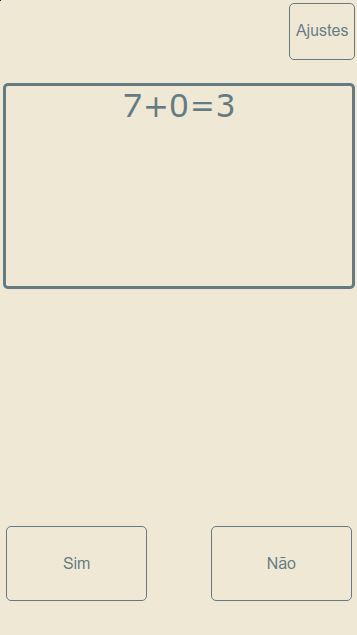
\includegraphics[width=0.8\textwidth,natwidth=610,natheight=642]{board.png}
	\caption{Interface do jogo com equação sendo apresentada}
    \label{fig:gameScreen}
\end{figure}

A construção da classe Match concebeu o comportamento principal do
jogo, entretanto, nesta etapa não havia um gerador de equações. O
jogo contava apenas com uma coleção de equações preestabelecidas que
eram selecionadas aleatoriamente a cada turno. Isso se provou uma boa
escolha pois possibilitou que o desenvolvimento se focasse em outros
aspectos importantes como a elaboração do laço do jogo, ranking,
configurações entre outros.

O ranking serve para armazenar o resultado de cada partida do jogador
possibilitando uma percepção de histórico da performance do jogador.
Os dados são armazenados em Local Storage, escolhido por ter uma API
simples. Arquiteturalmente falando, IndexedDb se encaixaria bem na
aplicação por ter uma interface chave valor, ideal para um ranking,
onde as chaves poderiam ser as posições do usuário. Não obstante,
a interface totalmente orientada a eventos do IndexedDb introduz uma
camada de complexidade desnecessária para os casos simples. Visto que
os requerimentos do protótipo não demandam grande performance ou
armazenamento massivo de dados a opção modesta, Local Storage,
foi preferida. A classe ranking é simplesmente uma interface para
converter partidas e armazenar e recuperas estas informações em Local
Storage. A figura \ref{fig:placar} demostra as informações do resultado
de uma partida bem como a posição do ranking.

%get a better image with better alignment
\begin{figure}
    \centering
    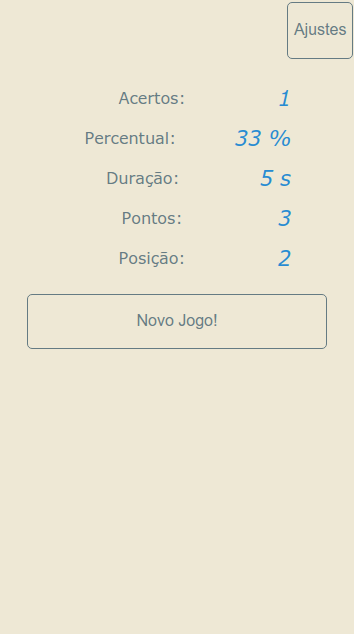
\includegraphics[width=0.8\textwidth,natwidth=610,natheight=642]{score.png}
	\caption{Resultado de uma partida}
    \label{fig:placar}
\end{figure}

O objeto \textit{Settings}, assim como o Ranking, utiliza Local Storage
e provê uma interface para armazenar e recuperar preferências sobre
o jogo. Cada campo editável na tela de configurações contém
\textit{listeners} prontos para registrar no objeto \textit{Settings}
cada mudança que ocorrer em seus estados. Os objetos que utilizam estas
configurações também o fazem através do objeto Settings, nunca
acessando configurações diretamente em Web Storage, dessa forma a
validade das configurações é garantida a a migração para uma forma
de armazenamento diferente é permitida com relativa facilidade.
A figura \ref{fig:configurations} demonstra a tela de configurações do 
jogo.

\begin{figure}
    \centering
    
\includegraphics[width=0.8\textwidth,natwidth=610,natheight=642]{settings.png}
	\caption{Configurações do jogo}
    \label{fig:cofigurations}
\end{figure}

Implementados estes mecanismos essenciais para o jogo, pude me
focar no ponto central do negócio e possivelmente o mais complexo:
a geração de equações. As geração das equações é feita
randomicamente envolve duas classes. Um objeto \textit{Statement},
responsável por armazenar as informações de uma equação, à dizer:
a afirmação sendo feita e se seu resultado está correto ou não (a
reposta da afirmação). O outro objeto envolvido neste processo é o
\textit{StatementGenerator}, responsável por gerar \textit{Statements}.

A classe \textit{StatementGenerator} conta com um método
\textit{getStatement} que realiza o processamento para gerar um
novo \textit{Statement}. Esta função recebe como argumento um
inteiro que simboliza a dificuldade da equação, a cada iteração
do usuário armazenada no objeto \textit{Match} a dificuldade é
incrementada e repassada para o gerador. O valor da dificuldade
é utilizado internamente no para selecionar qual operador será
utilizado e o tamanho do multiplicador dos números que compõem
as equações. Para colocar claramente: as equações são geradas
através da randomização de valores e operadores (com suas respectivas
dificuldades processadas), seguido da execução da equação para
determinar seu resultado e a geração, em 50\% dos casos, de um valor
errado, de modo que a resposta não seja sempre correta.

O objeto \textit{StatementGenerator} reside como membro de classe de
\textit{Match} e a cada interação com o usuário uma nova equação
é gerada por ele e armazenada no atributo \textit{currentStatement}
do objeto \textit{Match}. Ao final das iterações com o usuário o
evento \textit{endOfMatch} é lançado onde os pontos são computados,
armazenados e mostrados para o usuário. Neste ponto é possível
também começar outra partida reiniciando o processo.

Estas classes comportam os requisitos funcionais do jogo. Após um
período de uso, foi identificado que muitas vezes o usuário começa
uma partida e não está prestando atenção para a tela o que acarreta
na perda de pontos no período inicial da partida. Para reduzir este
problema foi adicionada a classe \textit{Countdown}, que é basicamente
um temporizador regressivo que demarca o início de cada partida,
notificando o usuário quanto falta para a partida iniciar. O temporizador foi
desenvolvido em canvas e apresenta 4 demarcações desenhadas a cada 90
graus, formando um circulo com uma mensagem no centro, neste caso os
números do temporizador. A  figura \ref{fig:counter} demonstra o contador 
prestes a iniciar uma nova partida.

\begin{figure}
    \centering
    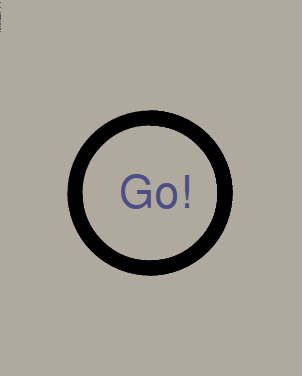
\includegraphics[width=0.8\textwidth,natwidth=610,natheight=642]{countdown.png}
	\caption{Contador em Canvas}
    \label{fig:counter}
\end{figure}

Para melhorar a experiência em desktops foram adicionados controles de
teclado além dos já presentes botões na interface, possibilitando que
o usuário utilize o teclado além do mouse. Quando o usuário utilizar
a seta para esquerda e direita os botões Sim e Não, respectivamente,
são clicados através de JavaScript. Simular o clique ao invés ao
invés de duplicar o tratamento das escolhas de resposta foi uma boa
estratégia pois centralizou o tratamento das respostas e evitou
duplicação.

\begin{draft}
%posteriori
Uma estratégia interessante que foi adotada na construção foi
declarar todos os objetos relativos ao objeto janela (\textit{window}).
Isso se demonstrou uma boa forma de separar os objetos, tornando o
conflito de variáveis globais um problema irrelevante.

Outro aspecto positivo foi a utilização de um meta objeto para
encapsular os demais, neste caso utilizei o nome MyMath, funcionando
como um namespace, garantindo que problemas de conflitos de nomes não
aconteçam.


\section{Performance}

O jogo ficou rápido...

\end{draft}
